\subsection{Контрольная работа №1, 14.11.2012}


%Теория вероятностей и математическая статистика. Контрольная работа 1, 14.11.12.

%\vspace{20pt}
%Обозначения: $\E(X)$ — математическое ожидание, $\Var(X)$ — дисперсия

\vspace{20pt}
14 ноября 1936 года в СССР была создана Гидрометеорологическая служба.
\vspace{20pt}

\begin{enumerate}

\item Погода завтра может быть ясной с вероятностью $0.3$ и пасмурной с вероятностью $0.7$. Вне зависимости от того, какая будет погода, Маша даёт верный прогноз с вероятностью $0.8$. Вовочка, не разбираясь в погоде, делает свой прогноз по принципу: с вероятностью $0.9$ копирует Машин прогноз, и с вероятностью $0.1$ меняет его на противоположный.
\begin{enumerate}
\item Какова вероятность того, что Маша спрогнозирует ясный день?
\item Какова вероятность того, что Машин и Вовочкин прогнозы совпадут?
\item Какова вероятность того, что день будет ясный, если Маша спрогнозировала ясный?
\item Какова вероятность того, что день будет ясный, если Вовочка спрогнозировал ясный?
\end{enumerate}

\item Машин результат за контрольную, $M$, равномерно распределен на отрезке $[0;1]$. Вовочка ничего не знает, поэтому списывает у Маши, да ещё может наделать ошибок при списывании. Поэтому Вовочкин результат, $V$, распределен равномерно от нуля до Машиного результата.
\begin{enumerate}
\item Найдите $\P(M>2V)$, $\P(M>V+0.1)$
\item Зачёт получают те, чей результат больше $0.4$. Какова вероятность того, что Вовочка получит зачёт? Какова вероятность того, что Вовочка получит зачёт, если Маша получила зачёт?
\end{enumerate}
Подсказка: попробуйте нарисовать нужные события в осях $(V,M)$

Это была задачка-неберучка!

\item Функция плотности случайной величины $X$ имеет вид $f(x)=\left\{\begin{array}{l}
\frac{3}{7}x^2,\, x\in[1;2] \\
0,\, x\notin [1,2]
\end{array}\right.$
\begin{enumerate}
\item Не производя вычислений найдите $\int_{-\infty}^{+\infty}f(x)\,dx$
\item Найдите $\E(X)$, $\E(X^2)$ и дисперсию $\Var(X)$
\item Найдите $\P(X>1.5)$
\item Найдите функцию распределения $F(x)$ и постройте её график
\end{enumerate}

\item Совместное распределение случайных величин $X$ и $Y$ задано таблицей

\begin{tabular}{@{}cccc@{}}
\toprule
      & $X=-2$ & $X=0$ & $X=2$ \\ \midrule
$Y=1$ & $0.2$  & $0.3$ & $0.1$ \\
$Y=2$ & $0.1$  & $0.2$ & $a$   \\ \bottomrule
\end{tabular}

\begin{enumerate}
\item Определите неизвестную вероятность $a$.
\item Найдите вероятности $\P(X>-1)$, $\P(X>Y)$
\item Найдите математические ожидания $\E(X)$, $\E(X^2)$
\item Найдите корреляцию $\Corr(X,Y)$
\end{enumerate}

\item Винни Пух собрался полакомиться медом, но ему необходимо принять решение, к каким пчелам отправиться за медом. Неправильные пчелы кусают каждого, кто лезет к ним на дерево с вероятностью 0.9, но их всего 10 штук. Правильные пчелы кусаются с вероятностью 0.1, но их 100 штук.
\begin{enumerate}
\item  Определите математическое ожидание и дисперсию числа укусов Винни Пуха для каждого случая
\item Определите наиболее вероятное число укусов и его вероятность для каждого случая
\item К каким пчелам следует отправиться Винни Пуху, если он не может выдержать больше двух укусов?
\end{enumerate}
\end{enumerate}



\subsection{Контрольная работа №1, 14.11.2012, решения}

\begin{enumerate}
\item
\begin{enumerate}
\item $\P(A)=0.8\cdot 0.3+0.7\cdot 0.2=0.38$
\item $\P(B)=0.9$
\item $\P(C|A)=\frac{0.3\cdot 0.8}{0.38}=0.632$
\item $\P(C|D)=\frac{0.3\cdot (0.9\cdot 0.8+0.1\cdot 0.2)}{0.9\cdot 0.38+0.1\cdot (1-0.38)}=0.55$
\end{enumerate}
\item Это была задачка-неберучка!
\item
\begin{enumerate}
\item $1$
\item $\E(X)=45/28\approx 1.61$, $\E(X^2)=93/35\approx 2.66$, $\Var(X)=291/3920\approx 0.07$
\item $37/56\approx 0.66$
\item $F(x)=\begin{cases} 0,\, x<1 \\
\frac{x^3-1}{7},\, x\in [1;2] \\
1,\, x>1 \end{cases}$
\end{enumerate}
\item
\begin{enumerate}
\item $a=0.1$
\item $\P(X>-1)=0.7$, $\P(X>Y)=0.1$
\item $\E(X)=-0.2$, $\E(X^2)=2$
\item $\Corr(X,Y)=0.117$
\end{enumerate}
\item
\begin{enumerate}
\item Правильные: $\E(X)=10$, $\Var(X)=9$, Неправильные: $\E(Y)=9$, $\Var(Y)=0.9$
\item Наиболее вероятное число укусов равно математическому ожиданию
\item Лучше идти к неправильным пчёлам, так как $\P(X\leq 2)<\P(Y\leq 2)$.
\end{enumerate}
\end{enumerate}


\subsection{Контрольная работа №2, 26.12.2012}

Тест:

\begin{enumerate}
\item Зная распределение компонент случайного вектора всегда можно восстановить их совместное распределение. Да. Нет.
\item Пусть $X$ — длина наугад выловленного удава в сантиметрах, а $Y$ — в дециметрах. Коэффициент корреляции между этими величинами равен 0.1. Да. Нет.
\item Для любой случайной величины $X$ справедливо неравенство
\[ \P(|X-\E(X)|>2\sqrt{\Var(X)})\leq 1/4 \]
Да. Нет.
\item Сумма независимых нормальных случайных величин нормальна. Да. Нет.
\item  Сумма $n$ независимых равномерно распределенных на интервале $(0,1)$ случайных величин асимптотически нормальна. Да. Нет.
\item Квадрат стандартной нормальной случайной величины имеет хи-квадрат распределение. Да. Нет.
\item Если ковариация компонент случайного двумерного нормального вектора равна нулю, то они независимы. Да. Нет.
\item Условная дисперсия всегда больше безусловной. Да. Нет.
\item Элементы выборки без возвращения из конечной генеральной совокупности независимы. Да. Нет.
\item Математическое ожидание выборочного среднего одинаково распределенных случайных величин не зависит от объема выборки. Да. Нет.
\item Конец света по техническим причинам переносится на показ работ по теории вероятности. Да. Может быть.
\end{enumerate}

Ответы: Нет, Нет, Да, Да, Да, Да, Да, Нет, Нет (зависимы), Да (не зависит), Любой верный

Задачи:
\begin{enumerate}
\item Купчиха Сосипатра Титовна очень любит чаёвничать. Её чаепитие продолжается случайное время $S$, имеющее равномерное распределение от 0 до 3 часов.  Встретив Сосипатру Титовну в пассаже на Петровке, её подруга Олимпиада Карповна узнала, сколько длилось вчерашнее чаепитие Сосипатры Титовны. Решив, что такая продолжительность чаепития является максимально возможной, Олимпиада Карповна устраивает чаепитие, продолжающееся случайное время $T$, имеющее равномерное распределение от 0 до $S$ часов.
\begin{enumerate}
\item Найдите совместную функцию плотности величин $S$ и $T$
\item Найдите вероятность $\P(S>T)$
\item Найдите $\E(T^2)$
\end{enumerate}

\item  Для случайно выбранного домохозяйства случайные величины $X$ и $Y$ принимают значения, равные доле расходов на продукты питания и алкоголь плюс табак соответственно. Случайный вектор $(X,Y)^T$  хорошо описывается двумерным нормальным законом распределения с математическим ожиданием $(0.45, 0.16)^T$ и ковариационной матрицей
\[
C=0.144\cdot
\left(\begin{array}{cc}
1 & -0.9 \\
-0.9 & 1
\end{array}\right)
\]
Найдите:
\begin{enumerate}
\item Вероятность того, что домохозяйство тратит более половины своих доходов на питание.
\item Вероятность того, что домохозяйство тратит более половины своих доходов на алкогольную и табачную продукцию и продукты питания.
\item Ожидаемую долю расходов на алкоголь и табак для домохозяйства, которое тратит на питание четверть своих доходов.
\item Вероятность того, что домохозяйство из предыдущего пункта тратит более трети своих доходов на алкогольную и табачную продукцию.

% из-за коррелированности этот пункт не решается :(
\begin{comment}
\item  Характеристикой отклонения от типичного потребления выступает величина
\[
U=\sqrt{\frac{(X-\E(X))^2}{\Var(X)}+\frac{(Y-\E(Y))^2}{\Var(Y)}}
\]
Найдите $\P(U>3)$.
\end{comment}
\item Для доли расходов на питание вычислите центральный момент 2013-го порядка.

\end{enumerate}

\item Вычислите (или оцените) вероятность того, что по результатам 4000 бросаний симметричной монеты,  частота выпадения герба будет отличаться от 0.5 не более, чем на $0.01$. Решите задачу с помощью неравенства Чебышёва и с помощью ЦПТ.


\item Компания кабельного телевидения НВТ, Новая Вершина Телевидения, анализирует возможность присоединения к своей сети пригородов N-ска. Опросы показали, что в среднем каждые 3 из 10 семей жителей пригородов хотели бы стать абонентами сети. Стоимость работ, необходимых для организации сети в любом пригороде оценивается величиной 2\,080\,000 у.е. При подключении каждого пригорода НВТ надеется получить 1\,000\,000 у.е. в год от рекламодателей. Планируемая чистая прибыль от оплаты за кабельное телевидение одной семьей в год равна 120 у.е.

Каким должно быть минимальное количество семей в пригороде для того, чтобы с вероятностью 0.99 расходы на организацию сети в этом пригороде окупились за год?


\item Оценки за контрольную работу по теории вероятностей 6 случайно выбранных студентов оказались равны:

8 5 6 7 3 9.

\begin{enumerate}
\item Выпишите вариационный ряд
\item Постройте график выборочной функции распределения
\item Вычислите значение выборочного среднего и выборочной дисперсии.
\end{enumerate}
\end{enumerate}

\subsection{Контрольная работа №2, 26.12.2012, решения}
\begin{enumerate}
\item  $f(s,t)=f(s)\cdot f(t|s)=\frac{1}{3s}$ при $0\leq t\leq s\leq 3$. Бонус тем, кто прочитал условие, $\P(S>T)=1$.
\[ \E(T^2)=\int_0^3\int_0^s \frac{t^2}{3s}\,dt\,ds=1 \]
\item
\begin{enumerate}
\item $\P(X>0.5)=\P(Z>0.1317616)\approx 0.4475864$, $\sigma_X\approx 0.3794733$
\item $\P(X+Y>0.5)=
\P(Z>-0.6481812)\approx 0.7415661$,
$\sigma_{X+Y}=0.1697056$, $\E(X+Y)=0.61$

\item $X=0.25$ при нормировке даёт $\tilde{X}=-0.5270463$. Получаем: $\E(\tilde{Y}\mid \tilde{X}=-0.5270463)=0.4743416$,  $\Var(\tilde{Y}\mid \tilde{X}=-0.5270463)=0.19$.

Значит $\E(Y \mid \tilde{X}=-0.5270463)=0.34$,  $\Var(Y\mid \tilde{X}=-0.5270463)=0.02736$.

\item $\P(Y>1/3\mid \tilde{X}=-0.5270463)=\P(Z>-0.0403042)=0.5160747$
\item Ноль
\end{enumerate}
\item $\E(\hat{p})=0.5$, $\Var(\hat{p})=0.25/n=1/16000$. По Чебышёву:
\[
\P(|\hat{p}-0.5|\leq 0.01)\geq 1-\frac{\Var(\hat{p})}{0.01^2}=\ldots=0.375
\]
Используя нормальную аппроксимацию:

\[
\P(|\hat{p}-0.5|\leq 0.01)=\P(|Z|\leq 1.2649111)\approx 0.7940968
\]
\item Обозначим $N$ — количество подключенных абонентов, тогда $N\sim Bin(n,0.3)$. При больших $n$ биномиальное распределение можно заменить на нормальное, $N\sim \cN(0.3n,0.21n)$.

\[ \P(120N>1\,080\,000)=\P(N>9000)=\P\left(Z>\frac{9000-0.3n}{\sqrt{0.21n}}\right)=0.99 \]

Из таблицы находим, что

\[ \frac{9000-0.3n}{\sqrt{0.21n}}=-2.3263479\]



Решаем квадратное уравнение, находим корни, один — отрицательный, другой, $n\approx 30622$.
\item



Вариационный ряд: 3, 5, 6, 7, 8, 9. $\bar{X}\approx 6.3333333$,
$\frac{\sum (X_i-\bar{X})^2}{n-1}\approx 4.6666667$,
$\frac{\sum (X_i-\bar{X})^2}{n}\approx 3.8888889$


\begin{minipage}{0.6\textwidth}
\begin{center}
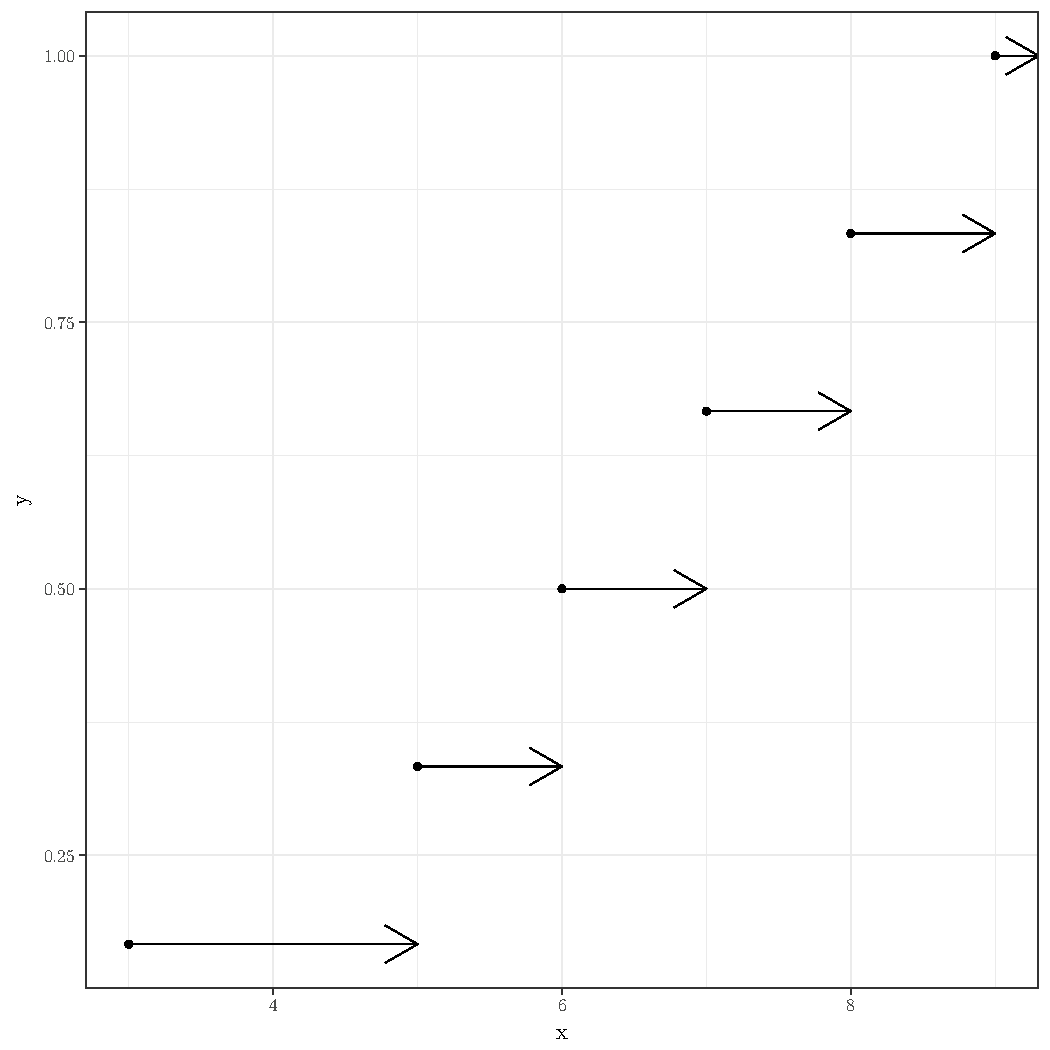
\includegraphics[scale=0.5]{auto_figures_tikz/2012_2013_fig_02_empirical_dist.pdf}
\end{center}
\end{minipage}


\end{enumerate}

\subsection{Демо-версия зачёта}

\begin{enumerate}
\item Двое подельников, Маша и Саша, украли десять миллионов евро. Через некоторое время Саша был найден убитым, а Маша была арестована. Из свидетельских показаний ясно следует, что Маша и Саша ругались по поводу делёжки. Защита и обвинение выясняют, убила ли Маша Сашу. Из статистических данных известно, что:
\begin{enumerate}
\item[A] 20\% подельников-мужчин ругаются по поводу делёжки
\item[B] 20\% оставшихся в живых подельников-мужчин ругаются по поводу делёжки
\item[C] 5\% мужчин убивают
\item[D] 3\% мужчин убивают их подельники
\item[E] 90\% убитых мужчин-подельников ругались по поводу делёжки
\end{enumerate}
Располагая этой информацией,
\begin{enumerate}
\item Найдите вероятность того, что Маша убила Сашу, если известно, что Маша и Саша ругались по поводу делёжки.
\item Найдите вероятность того, что Маша убила Сашу, если известно, что Маша и Саша ругались по поводу делёжки, и Саша был найден убитым.
\end{enumerate}


\item Маша подкидывает 300 игральных кубиков. Те, что выпали не на шестёрку, она перекидывает один раз. Обозначим буквой $N$ количество шестёрок на всех кубиках после возможных перекидываний.
\begin{enumerate}
\item Найдите $\E(N)$, $\Var(N)$
\item Какова примерно вероятность того, величина $N$ лежит от 50 до 70?
\item Укажите любой интервал, в который величина $N$ попадает с вероятностью 0.9
\end{enumerate}

\item На лукоморье набегают волны. Кот Учёный заметил, что размер каждой волны, $X_i$, — случайная величина, имеющая равномерное распределение от 0 до 1, а размеры волн независимы. Кот Учёный считает волну \textit{большой}, если она больше предыдущей и следующей. Случайная величина $R_i$ равна 1, если $i$-ая волна была \textit{большой}, и 0 иначе.
\begin{enumerate}
\item Найдите $\P(R_i=1)$, $\E(X_i)$
\item Найдите $\E(X_i \mid R_i=1)$
\item Найдите $\Cov(R_1,R_2)$, $\Cov(R_1,R_3)$
\end{enumerate}
\item Ермолай Лопахин решил приступить к вырубке вишневого сада. Однако выяснилось, что растут в нём не только вишни, но и яблони. Причём, по словам Любови Андреевны Раневской, среднее количество деревьев (а они периодически погибают от холода или жары, либо из семян вырастают новые) в саду распределено в соответствии с нормальным законом ($X$ — число яблонь, $Y$ — число вишен) со следующими параметрами:
\begin{equation*}
\begin{pmatrix}	X \\ 	Y 	\end{pmatrix}
\sim \mN
\left(
\begin{pmatrix}
25 \\ 125
\end{pmatrix}
;
\begin{pmatrix}
    5 & 4 \\
    4 & 10
    \end{pmatrix}
\right)
\end{equation*}

\begin{enumerate}
\item Найдите вероятность того, что Ермолаю Лопахину придется вырубить более 150~деревьев.
\item Каково ожидаемое число подлежащих вырубке вишен, если известно, что предприимчивый и последовательный Лопахин, не затронув ни одного вишнёвого дерева, начал очистку сада с яблонь и все 35~яблонь уже вырубил? Какова при этом вероятность того, что Лопахину придется вырубить более 100 вишен?
\end{enumerate}

\item Вопрос из интервью в Морган-Стэнли. Есть две независимых равномерных на отрезке $[0;1]$ случайных величины, $X$ и $Y$. Как их нужно преобразовать, чтобы корреляция между ними оказалась равна $\rho$?
\end{enumerate}

\subsection{Зачёт, 15.01.2013}


\begin{enumerate}
\item Самолёт упал либо в горах, либо на равнине. Вероятность того, что самолёт упал в горах, равна 0.75. Для поиска пропавшего самолёта выделено 3 вертолёта. Каждый вертолёт можно использовать только в одном месте. Как распределить имеющиеся вертолёты, если вероятность обнаружения пропавшего самолёта отдельно взятым вертолётом равна $0.6$?

\item Совместная функция плотности величин $X$ и $Y$ имеет вид
\[
f(x,y)=\frac{1}{x}e^{-x},\: \text{при}\: 0<y<x
\]

\begin{enumerate}
\item Найдите $\P\left( \frac{Y}{X}<0.7 \right)$
\item Найдите $\E(X)$
\item Являются ли $X$ и $Y$ независимыми?
\item Как распределена величина $Z=Y/X$?
\end{enumerate}

\item Величины $X_1$, \ldots, $X_n$ независимы и имеют биномиальное распределение, $X_i \sim Bin(10,p)$. Используя неравенство Чебышёва найдите наименьшее число $t$, чтобы выполнялось условие
\[
\P( | \bar{X}-\E(\bar{X}) | \geq t )\leq 0.01
\]



\item Допустим, что срок службы пылесоса имеет экспоненциальное распределение. В среднем один
пылесос бесперебойно работает 10 лет. Завод предоставляет гарантию 7 лет на свои изделия.
Предположим для простоты, что все потребители соблюдают условия гарантии.
\begin{enumerate}
\item Какой процент потребителей в среднем обращается за гарантийным ремонтом?
\item Какова вероятность того, что из 1000 потребителей за гарантийным ремонтом обратится
более 55\% покупателей?
\end{enumerate}
Подсказка: $\ln 2\approx 0.7$

\item Вася попадает мячом в корзину с вероятностью $0.2$, Петя — с вероятностью $0.25$. Каждый из них сделал по 100 бросков мяча.
\begin{enumerate}
\item Какова вероятность того, что Петя попал на 10 раз больше Васи?
\item Какое минимальное количество бросков мяча нужно сделать каждому, чтобы вероятность, того, что Петя попал на 10 раз больше Васи достигла 0.99?
\end{enumerate}
\end{enumerate}

\subsection{КоКо, компьютерная контрольная №3, 13.03.13}

Продолжительность 1 час 10 минут, разрешено пользоваться конспектами, книжками, заготовками программ, нельзя общаться, использовать Интернет. Текст работы в группах с R:

\begin{enumerate}
\item Величины $X$ и $Y$ независимы. Величина $X$ распределена нормально, $X\sim \cN(4.4, 6.5)$, величина $Y$ распределена экспоненциально, $Y\sim \exp(\lambda=2.3)$. Используя симуляционный подход примерно посчитайте

\begin{enumerate}
\item $\P(X+Y>5.2)$
\item $\E(X/(X+6Y))$
\item $\Var(XY)$
\item $\Cov(XY,X/Y)$
\end{enumerate}

\item Загрузите данные по стоимости квартир в Москве, \href{http://goo.gl/zL5JQ}{goo.gl/zL5JQ}, в табличку с именем \verb|h|. Обозначим буквой \verb|a| ответ на первый вопрос первой задачи. Отберите индивидуальную выборку лично для себя, выполнив команды:

\begin{minted}[mathescape,
               linenos,
               numbersep=5pt,
               frame=lines,
               framesep=2mm]{r}
set.seed(round(100 * a)) # здесь "a" — это ответ на первый пункт первой задачи
h <- h[sample(1:nrow(h), 1000), ]
\end{minted}

Постройте 90\%-ый доверительный интервал для:
\begin{enumerate}
\item Доли кирпичных домов, \verb|brick==1|
\item Доли кирпичных домов, \verb|brick==1|, среди домов находящихся близко от метро,  \verb|walk==1|
\item Разницы доли кирпичных домов среди домов расположенных близко и далеко от метро
\end{enumerate}


\item Сгенерируйте искусственные данные, выполнив команды:
\begin{minted}[mathescape,
               linenos,
               numbersep=5pt,
               frame=lines,
               framesep=2mm]{r}
set.seed(round(100 * a) + 42) # здесь "a" — это ответ на первый пункт первой задачи
x <- rexp(200, rate = 2)
\end{minted}

Величины $X_i$ независимы и имеют функцию плотности $f(x)=e^{b-xe^b}$ при $x>0$.
\begin{enumerate}
\item Оцените неизвестный параметр $b$
\item Оцените дисперсию полученной оценки
\item Постройте 90\%-ый доверительный интервал для $b$
\item Используя результат предыдущего пункта, на 10\%-ом уровне значимости проверьте гипотезу $H_0$: $b=0.7$ против альтернативной гипотезы $H_a$: $b\neq 0.7$.
\end{enumerate}

\end{enumerate}


\subsection{Экзамен, 26.03.2013}


\begin{enumerate}
%в комментариях предполагаемые ответы


\item Вероятность выигрыша по лотерейному билету равна $0.05$. Вероятность того, что из трёх купленных билетов ровно два окажутся выигрышными примерно равна

\otvet{0.002}{0.0025}{0.007}{0.1}{0.3}

\item Закон распределения случайной величины задан табличкой

\begin{tabular}{@{}cccc@{}}
\toprule
$x$         & $-1$  & $0$   & $1$ \\ \midrule
$\P(X=x)$ & $0.4$ & $0.2$ & ?   \\ \bottomrule
\end{tabular}

Дисперсия величины $X$, $\Var(X)$, равняется

\otvet{0}{0.02}{0.3}{0.8}{2}

%3
\item Если $f(x)$ — функция плотности, то $\int_{-\infty}^{x}f(u)\,du$ равен

\otvet{0}{1}{$\E(X)$}{$\Var(X)$}{$F(x)$}

%4
\item События $A$ и $B$ называются независимыми, если

\lotvet{$\P(A\cup B)=\P(A)+\P(B)$}
{$\P(A)\cdot\P(B)=\P(A\cap B)$}
{$\P(A\cup B)=\P(A)+\P(B)-\P(A\cap B)$}
{$\P(A\cap B)=0$}
{нет верного} \\ \\

%5
\item Правильную монетку подбрасывают два раза. Рассмотрим два события: $A$ — при втором броске выпала «решка», $B$ — «орёл» выпал хотя бы один раз. Найдите $\P(A|B)$

\otvet{0}{1/3}{1/2}{2/3}{1}

%6
\item Есть пять случайных величин: $X\sim \chi^2_{10}$, $Y\sim F_{5,10}$, $T\sim t_{10}$, $Z\sim \cN(0,1)$, $W\sim \cN(10,1)$. Какие из величин распределены симметрично относительно 0?

\otvet {X, Y, Z}{Z, W}{Z, T}{Z}{X, Y}

%7
\item Известно, что $\E(X)=3$, $\Var(X)=1$, $\E(Y)=4$, $\Var(Y)=9$, $\E(XY)=13$, найдите $\Cov(X,Y)$

\otvet{0}{-3}{18}{3}{1}

%8
\item Известно, что $\E(X)=3$, $\Var(X)=1$, $\E(Y)=4$, $\Var(Y)=9$, $\E(XY)=6$, найдите $\Var(2X+Y)$

\otvet{13}{7}{1}{17}{нет верного ответа}

%9
\item Если $F(x)$ — это функция распределения, то $\lim_{x\to -\infty}F(x)$ равен

\otvet{0}{0.5}{1}{$\E(X)$}{$+\infty$}

%10
\item Если $X\sim \cN(-4;1)$, то $\P(3X+571>0)$ примерно равна

\otvet{0}{0.5}{1}{$+\infty$}{нет верного ответа}

%11
\item Про закон распределения величины $X$ ничего не известно. Укажите самую точную оценку сверху для вероятности $\P(|X-\E(X)|>3\sqrt{\Var(X)})$

\otvet{$0.(3)$}{$0.6(3)$}{$0.(1)$}{$1$}{нет верного ответа}

%12
\item Функция распределения, $F(x)=\P(X\leq x)$ может не являться

\otvet{непрерывной}{непрерывной справа}{монотонно неубывающей}{ограниченной}{неотрицательной}

%13
\item Ковариационной может быть матрица:

\otvet {$\left(\begin{array}{cc}
-1 & 1\\
1 & 2
\end{array}\right)$}{$\left(\begin{array}{cc}
1 & 0.5\\
1 & 2
\end{array}\right)$}{$\left(\begin{array}{cc}
1 & -1\\
-1 & 2
\end{array}\right)$}{$\left(\begin{array}{cc}
-1 & 1\\
1 & -2
\end{array}\right)$}{$\left(\begin{array}{cc}
1 & 1\\
-0.7 & 2
\end{array}\right)$}\\

%14
\item Если $X$ и $Y$ независимые случайные величины, то неверным может быть утверждение

\lotvet{$\E(X+Y)=\E(X)+\E(Y)$}
{$\E(X/Y)=\E(X)/\E(Y)$}
{$\E(XY)=\E(X)\cdot\E(Y)$}
{$\Var(X+Y)=\Var(X)+\Var(Y)$}
{$\Cov(X,Y)=0$} \\ \\

%15
\item Известно, что  $\Cov(X,Y)=0$, $\Var(X)=10$, $\Var(Y)=10$. \\
Неверным может быть утверждение

\lotvet{$\Corr(X,Y)=0$}
{$\Corr(X+a,Y+b)=0$}
{$\E(X\cdot Y)=\E(X)\cdot \E(Y)$}
{$\Var(X+Y)=\Var(X)+\Var(Y)$}
{$X$ и $Y$ независимы} \\ \\

%16
\item $Z_1,Z_2,\ldots,Z_n\sim\cN(0,1)$. Тогда величина $\frac{Z_1\sqrt{n-2}}{\sqrt{\sum_{i=3}^n Z_i^2}}$ имеет распределение

\otvet {$\cN(0,1)$}{$t_n$}{$F_{1,n-2}$}{$\chi^2_n$}{$t_{n-2}$}

%17
\item Количество страниц в книгах авторов $X$ и $Y$ распределено нормально с дисперсиями $\sigma^2_X$ и $\sigma^2_Y$ соответственно. Для тестирования гипотезы о равенстве дисперсий было выбрано $n$ книг автора $X$ и $m$ книг — автора $Y$. Какое распределение имеет статистика, используемая в данном случае?

\otvet {$\chi^2_{\min(m,n)}$}{$\chi^2_{\max(m,n)}$}{$F_{m,n}$}{$F_{m-1,n-1}$}{$F_{m+1,n+1}$}

%18
\item Если величина $X$ имеет $\chi^2_k$-распределение, величина $Y$ — $\chi^2_n$-распределение, и они независимы, то дробь $nX/(kY)$ имеет распределение

\otvet{$F_{k,n}$}{$F_{n,k}$}{$F_{k-1,n-1}$}{$\chi^2_{n-k}$}{$F_{n-1,k-1}$}

%19
\item \emph{Смещённой} оценкой математического ожидания по выборке независимых,
одинаково распределенных случайных величин $X_1$, $X_2$, $X_3$ является оценка

\lotvet{$(X_1+X_2)/2$}{$(X_1+X_2+X_3)/3$}{$0.7X_1+0.2X_2+0.1X_3$}{$0.3X_1+0.3X_2+0.3X_3$}{$X_1+X_2-X_3$} \\ \\

%20
\item Если величины $X$ и $Y$ независимы и равномерно распределены на $[0;1]$, а $F(x,y)$ — их совместная функция  распределения, то $F(0.5,3)$ равно

\otvet{0}{0.5}{1}{1.5}{не существует}

%21
\item Если $X_i$ независимы и имеют нормальное распределение $\cN(-1;2013)$, то $\sqrt{n}(1+\bar{X})/\hat{\sigma}$ имеет распределение

\otvet{$\cN(0;1)$}{$t_{n-1}$}{$\chi^2_{n-1}$}{$\cN(0;2013/n)$}{$t_n$}

%22
\item Последовательность оценок $\hat{\theta}_1$, $\hat{\theta}_2$, \ldots называется состоятельной, если

\lotvet{$\E(\hat{\theta}_n)=\theta$}{$\Var(\hat{\theta}_n)\to 0$}{$\P(|\hat{\theta}_n - \theta |>t)\to 0$ для всех $t>0$}{$\E(\hat{\theta}_n)\to \theta$}
{$\Var(\hat{\theta}_n)\geq \Var(\hat{\theta}_{n+1})$} \\ \\

%23
\item Величины $X_1$, \ldots, $X_5$ равномерны на отрезке $[0;a]$. Известно, что $\sum_{i=1}^5 x_i=25$. При использовании первого момента оценка методом моментов неизвестного $a$ равна

\otvet{1}{5}{10}{20}{нет верного ответа}

%24
\item При построении доверительного интервала для отношения дисперсий по двум независимым нормальным выборкам из $n$ наблюдений каждая, используется статистика, имеющая распределение

\otvet{$F_{n-1,n-1}$}{$t_{n-1}$}{$\chi^2_{n-1}$}{$\chi^2_{n}$}{$t_n$}

%25
\item Ботаники\footnote{В отличие от ботаников, зоологи точно знают, сколько иголок у ёжиков!} строят доверительный интервал для математического ожидания числа иголок у ёжа. Количество иголок на одном еже предполагается нормально распределенным. Среднее число иголок у пойманных 100 ёжиков равно 1500, выборочная дисперсия — 400. На 5\% уровне значимости какой примерно доверительный интервал должны построить ботаники?


\lotvet {$[1499;1501]$}{$[1498;1502]$}{$[1497;1503]$}{$[1496;1504]$}{нет верного ответа}\\ \\

%26
\item Функция правдоподобия, построенная по случайной выборке $X_1$, \ldots, $X_n$ из распределения с функцией плотности $f(x)=(\theta+1)x^{\theta}$ при $x\in [0;1]$ имеет вид

\otvet{$(\theta+1)x^{n\theta}$}{$\sum (\theta+1)x_i^{\theta}$}
{$(\theta+1)^{\sum x_i}$}{$(\sum x_i)^{\theta}$}{$(\theta+1)^n\prod x_i^{\theta}$}

%27
\item Если $X_i$ независимы, $\E(X_i)=\mu$ и $\Var(X_i)=\sigma^2$, то математическое ожидание величины $Y=\sum_{i=1}^{n}(X_i-\bar{X})^2$ равно

\otvet{$\hat{\sigma}^2$}{$(n-1)\sigma^2$}{$\mu$}{$\sigma^2$}{$\sigma^{2}/n$}

%28
\item Если $P$-значение меньше уровня значимости $\alpha$, то гипотеза $H_0$: $\sigma=\sigma_0$

\lotvet{отвергается}{не отвергается}{отвергается только если $H_a$: $\sigma \neq \sigma_0$}{отвергается только если $H_a$: $\sigma<\sigma_0$}{недостаточно информации} \\

\item Если $H_0$ верна, то $P$-значение имеет распределение

\otvet{$U[0;1]$}{$\cN(0,1)$}{$t_n$}{$t_{n-1}$}{$\chi^2_{n-1}$}


\end{enumerate}


\textbf{Экзамен по теории вероятностей! Суперигра!}

\vspace{20pt}
\begin{center}
\textbf{DON'T PANIC}
\end{center}
\vspace{20pt}


\begin{enumerate}
\item В группе учится 30 студентов, 20 девушек и 10 юношей. Они входят в аудиторию в случайном порядке. Рассчитайте вероятности событий:
\begin{enumerate}
\item Маша Петрова\footnote{Маша Петрова — единственная и неподражаемая!} войдёт девятой по счёту
\item Девятый вошедший окажется девушкой
\item Перед Машей Петровой войдут ровно 5 юношей
\item Перед Машей Петровой войдут ровно 5 юношей, если известно, что Маша Петрова вошла девятой
\item Маша Петрова войдёт девятой по счёту, если известно, что перед ней вошло ровно 5 юношей
\end{enumerate}

\item В поселке 2500 жителей. Каждый из них в среднем 6 раз в месяц ездит в город, выбирая день поездки независимо от других людей. Поезд ходит в город один раз в сутки.
\begin{enumerate}
\item Какой наименьшей вместимостью должен обладать поезд, чтобы он переполнялся в среднем не чаще 1 раза в 100 дней?
\item Сколько в среднем человек будет ехать в таком поезде, если предположить, что при переполнении часть людей полностью откажется от поездки?
\end{enumerate}

Источник: экзамен РЭШ

\item Случайные величины $X_1$, $X_2$, \ldots, $X_n$ независимы и имеют пуассоновское распределение с неизвестным параметром $\lambda$.
\begin{enumerate}
\item С помощью метода максимального правдоподобия постройте оценки для $\lambda$ и для $\exp(\lambda)$
\item Предположим, что исследователь не знает, чему равны $X_i$. Ему известно лишь, равно ли каждое из $X_i$ нулю или нет. С помощью метода максимального правдоподобия постройте оценки для $\lambda$ и для $\exp(\lambda)$. Всегда ли существуют предложенные оценки?
\end{enumerate}


\item В таблице представлены данные по количеству пассажиров «Титаника», поделенные на группы по классу каюты:

\begin{table}[ht]
\centering
\begin{tabular}{rrrr}
  \toprule
 & 1 класс & 2 класс & 3 класс \\
  \midrule
Погиб & 122 & 167 & 528 \\
  Выжил & 203 & 118 & 178 \\
   \bottomrule
\end{tabular}
\end{table}

Проверьте гипотезу о независимости шансов выжить от класса каюты.

\item Перед Вами две внешне неотличимых монетки. Одна из них выпадает «орлом» вверх с вероятностью $0.7$, другая — с вероятностью $0.3$. Вы имеете право на 4 подбрасывания. Перед каждым подбрасыванием Вы можете выбирать подбрасываемую монетку. За каждого выпавшего «орла» вы получаете 1 рубль.
\begin{enumerate}
\item Какова оптимальная стратегия?
\item Каков ожидаемый выигрыш при использовании оптимальной стратегии?
\end{enumerate}

\end{enumerate}
